\section{Privacy}
The current banking system achieves a level of privacy by keeping key information hidden from the public. Under this regime, all identities are known by the trusted third party, i.e. the bank.

In the Tagion system, all transactions and bills are public, but physical identities are separated from transactions and bills. The system has full transparency regarding how many bills exist. A public key is bound to a bill and not an account, and the private key is for signing and spending the bill.\\

\begin{figure}[H]
 \centering
 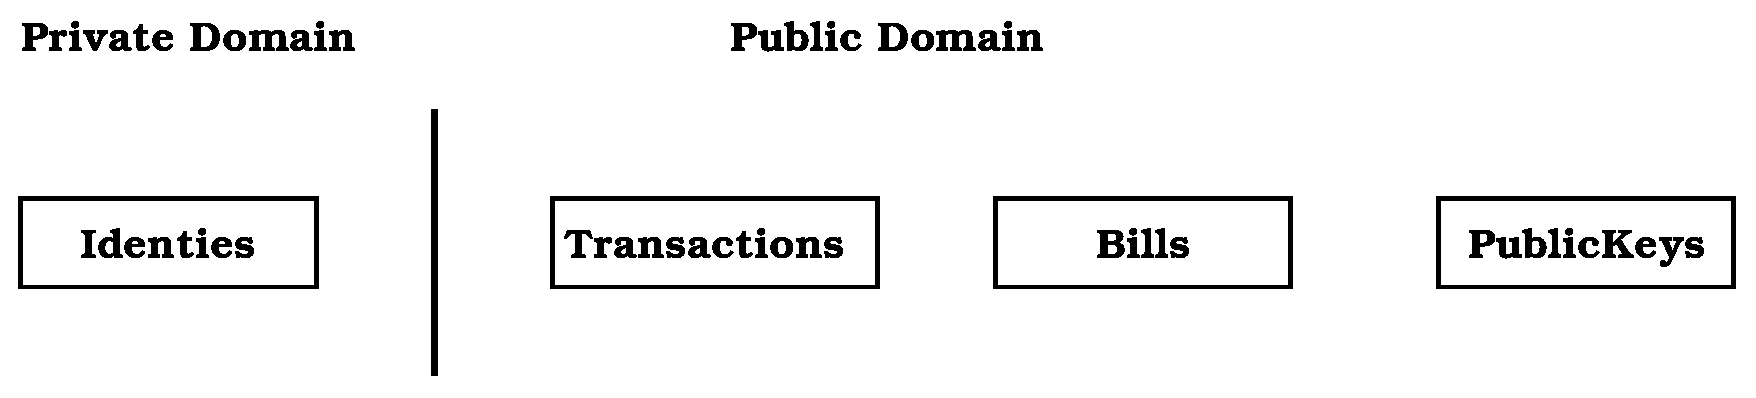
\includegraphics[width=0.8\textwidth]{fig/privacy.eps}
 \caption{Private and Public domain}
 \label{fig:private_domain}
\end{figure}

Tagion bills are not linked in a chain because each time a bill is spent, a transaction is recorded in the database, deleting the old bill and creating a new one. A full trace of the network will, however, reveal the inputs and outputs of transactions, thus linking the bills. Over time, the bills split and re-combine as they become part of multiple in and out transactions. Therefore, it is not feasible to search back through the linking of bills for a pattern, because it is not a 1:1 trace of bills and would cause an NP (non-polynomial) problem, which cannot be solved in finite time.\\

\begin{figure}[H]
 \centering
 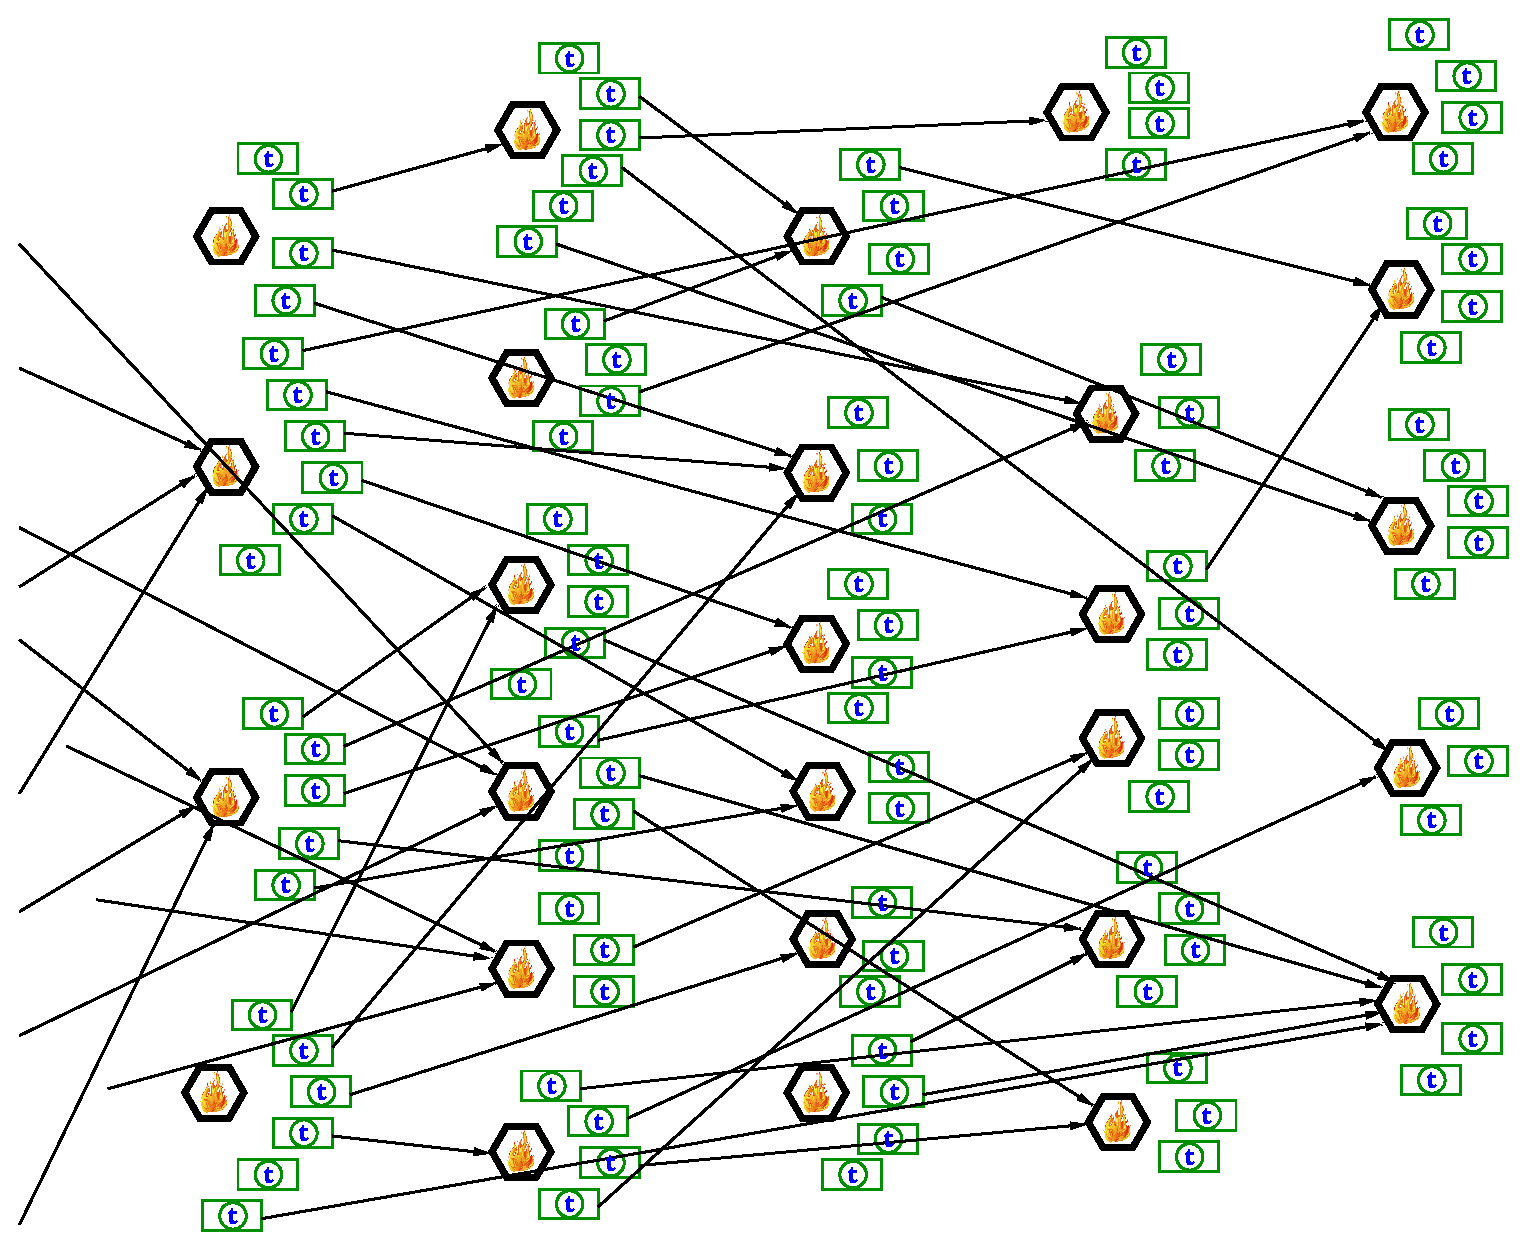
\includegraphics[width=0.9\textwidth]{fig/transaction_inout.eps}
 \caption{A transaction is represent as a hexagon with a flame the small-bank-note with a {\bfseries{t}} represent bills}
 \label{fig:transaction_inout}
\end{figure}

A user can determine if the same public key should be the owner of all his/her bills or a different, derived, public key. They can hold a different public key for each owned bill, and these keys may not correlate with each other. By using a different public key for each node, a user can make transactions in full privacy, i.e. anonymously.\\ 
A node is a public servant and therefore needs to reveal public information. A node in the Tagion system needs to use a fixed public key to ensure the governance of the node. The public key is the identifier for the node that can be perceived as an account, and it is the account for receiving rewards.\\ 
